\documentclass[11pt]{beamer}
%\usetheme{PaloAlto}
\usetheme{Warsaw}
\usepackage[utf8]{inputenc}
\usepackage{amsmath}
\usepackage{amsfonts}
\usepackage{amssymb}
\usepackage{listings}
\usepackage{color}


\usepackage[font=scriptsize]{caption}
\usepackage{mwe}

\setbeamercolor{institute in head/foot}{parent=palette primary}


\lstdefinestyle{customasm}{
  belowcaptionskip=1\baselineskip,
  frame=L,
  xleftmargin=\parindent,
  basicstyle=\footnotesize\ttfamily,
  commentstyle=\itshape\color{purple!40!black},
}

\lstdefinestyle{customc}{
  belowcaptionskip=1\baselineskip,
  breaklines=true,
  frame=L,
  xleftmargin=\parindent,
  language=R,
  showstringspaces=false,
  basicstyle=\footnotesize\ttfamily,
  keywordstyle=\bfseries\color{green!40!black},
  commentstyle=\itshape\color{purple!40!black},
  identifierstyle=\color{blue},
  stringstyle=\color{orange},
  numbersep=7pt
}



\graphicspath{{pictures/}}
\DeclareGraphicsExtensions{.pdf,.png,.jpg}

\author{Isabella Aspodinger, Alexander Pilan}
\title{Big Data}
\setbeamercovered{transparent} 
\setbeamertemplate{navigation symbols}{} 
%\logo{} 
\institute{Paris Lodron Universität Salzburg} 
\date{22. November, 2019} 
%\subject{} 
\begin{document}

\begin{frame}
\titlepage
\end{frame}

\begin{frame}{Inhalt}
\tableofcontents
\end{frame}

\begin{frame}{Allgemein}
\section{Allgemein}
\begin{figure}[h]
		\center{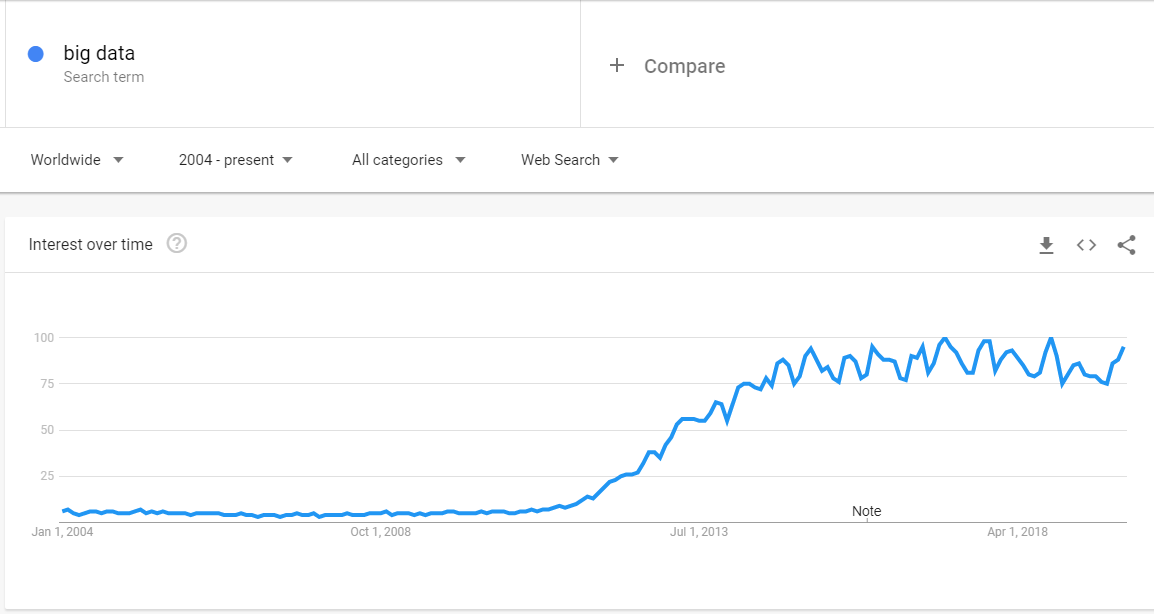
\includegraphics[scale=0.3]{bdtrend}}
		\caption{https://trends.google.com/trends/}
		\label{ris:image}
	\end{figure}
\end{frame}


\begin{frame}{Definition}
\subsection{Definition}


	\begin{itemize}
	\item Volume (Datenvolumen)
	\item Velocity (Geschwindigkeit der Datenverarbeitung und Veränderungsdynamik)
	\item Variety (Vielfalt der Datenstrukturen und -klassen)
	\item Veracity (Echtheit der Daten)
	\item Value (unternehmerischer Mehrwert)
	\item Validity (Datenqualität)
	\end{itemize}




\end{frame}

\begin{frame}{Unterschied}
\subsection{Unterschied}
\setlength\tabcolsep{0pt}
\setlength\thickmuskip{0mu}
\setlength\medmuskip{0mu}
\small
\centering
\begin{tabular*}{\textwidth}{ p{145pt} p{145pt}} 
Traditionelle Analytik & Big Data Analytik \\ 
\begin{itemize}
\item Schrittweise Analyse von kleinen Datenmengen
\item Daten werden angesammelt, bearbeitet, gespeichert und erst dann analysiert 
\end{itemize}
&
\begin{itemize}
\item Bearbeitung der ganzen Datenmenge 
\item Daten werden unverändert bearbeitet
\item Analyse und Bearbeitung werden je nach Eingang durchgeführt 
\end{itemize}

\end{tabular*} 
	%\begin{figure}
		%\center{\includegraphics[scale=0.35]{}}
	%	\end{figure}
\end{frame}

\begin{frame}{Datenherkunft}
\subsection{Datenherkunft}
\begin{enumerate}
\item Aufzeichnungen verschiedenster Überwachungssysteme.
\item die Nutzung von Kunden- oder Bank- bzw. Bezahlkarten 
\item die Nutzung eines Smartphones
\item Social-Media
\item Kraftfahrzeuge
\item vernetzte Technik in Häusern
\item von Behörden und Unternehmen erhobene und gesammelte Daten.
\end{enumerate}
\end{frame}

\begin{frame}{Wachstum von Daten}
\subsection{Wachstum von Daten}
	\begin{figure}
		\center{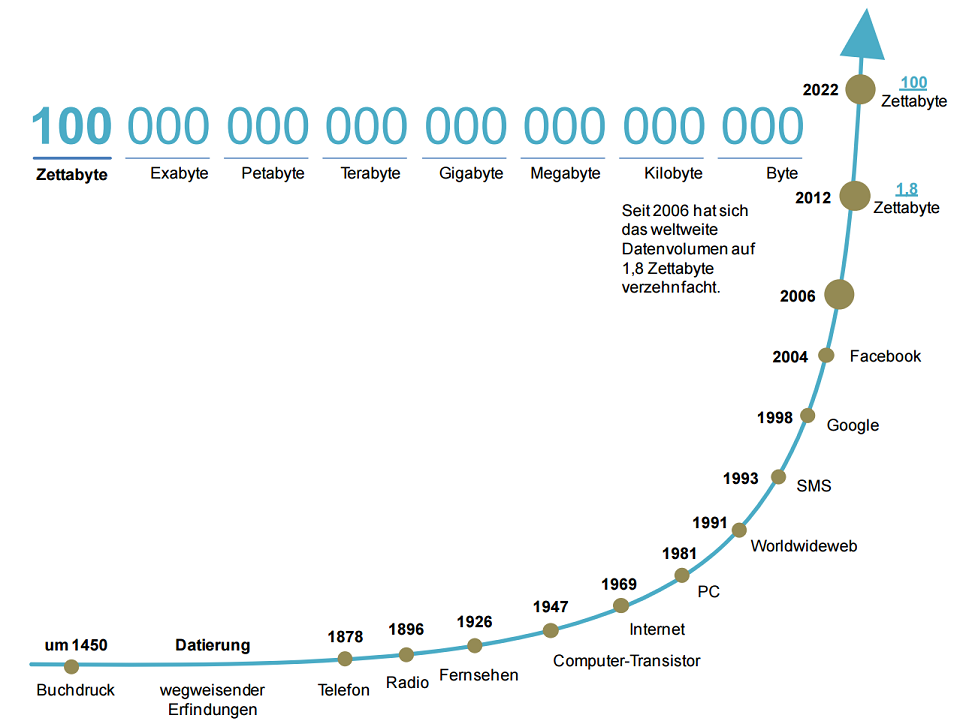
\includegraphics[scale=0.31]{bigdatapng1}}
		\caption{https://bigdatablog.actgruppe.de/2017/04/06/die-geschaeftliche-herausforderung-von-big-data/}
	\end{figure}
\end{frame}

\begin{frame}{Anwendung}
\subsection{Anwendung}
%https://piwikpro.de/blog/was-ist-big-data-und-wie-profitieren-unternehmen-davon/
	\begin{enumerate}
		\item Wahlen 
		\item Social Scoring
		\item Bildungswesen
		\item Wirtschaft
		\item Staat
		\item Gesundheit
		\item Umwelt
	\end{enumerate}
\end{frame}



\begin{frame}{Analysemethoden}
\section{Analysemethoden}
\begin{itemize}
\item Repräsentative Stichprobe
\item Kopplungsanalyse
\item Predictive Analytics
\end{itemize}
\end{frame}

\begin{frame}{Entwicklungen}
\section{Entwicklungen}
	\begin{itemize}
	\item NOSQL (Not Only SQL)
	\item JSON 
	\item Map Reduce
	\item Hadoop
	\item Spark
	\item R
	\end{itemize}
\end{frame}


\begin{frame}{Kopplungsanalyse}
\begin{figure}
		\center{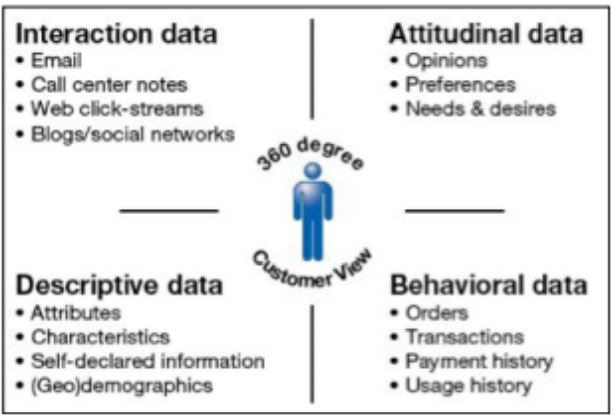
\includegraphics[scale=0.5]{img5}}
	\end{figure}
\end{frame}

%
%\begin{frame}{Schwerpunkte}
%\subsection{Schwerpunkte}
%\begin{itemize}
%\item Verarbeitung vieler Datensätze
%\item Verarbeitung vieler Spalten innerhalb eines Datensatzes
%\item Schneller Import großer Datenmengen
%\item Sofortige Abfrage importierter Daten (Realtime Processing)
%\item Kurze Antwortzeiten (Latenz und Verarbeitungsdauer) auch bei komplexen %Abfragen
%\item Möglichkeit zur Verarbeitung vieler gleichzeitiger Abfragen (Concurrent %Queries)
%\item Analyse verschiedenartiger Informationstypen (Zahlen, Texte, Bilder, …)
%\end{itemize}
%\end{frame}

\begin{frame}{NoSQL}
\subsection{NoSQL}
\begin{itemize}
\item Objektdatenbanken
\item Grid- und Cloud-Datenbanken
\item XML-Datenbanken
\item Andere nicht-relationale Datenbanken
\end{itemize}
\end{frame}

\begin{frame}{NoSQL}
\framesubtitle{Kriterien}
\begin{itemize}
\item Nichtrelationales Datenmodell
\item Schemafrei (oder nur schwache Restriktionen)
\item Bieten einfache API
\item Verteilte Architektur, optimiert für einfache Replikation 
\item Skalierung
\item Kein ACID-Konsistenzmodell
\item Open Source
\end{itemize}
\end{frame}

\begin{frame}{NoSQL}
\begin{figure}
		\center{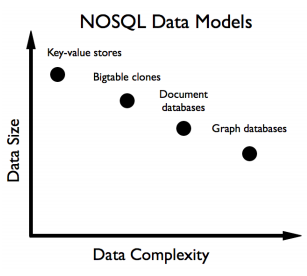
\includegraphics[scale=0.5]{img2}}
		\caption{https://www.slideshare.net/timjuravich/mysql-nosql-from-a-php-perspective}
\end{figure}
\end{frame}

\begin{frame}[fragile]
\frametitle{JavaScript Object Notation}
\subsection{JSON}
JSON ist ein kompaktes Datenformat in einer einfach lesbaren Textform zum Zweck des Datenaustauschs zwischen Anwendungen.


\lstset{
	showtabs=false,
	basicstyle=\footnotesize\ttfamily\color{black}
}
\begin{lstlisting}
{
  "Herausgeber": "Xema",
  "Nummer": "1234-5678-9012-3456",
  "Deckung": 2e+6,
  "Waehrung": "EURO",
  "Inhaber": {
    "Name": "Mustermann",
    "Vorname": "Max",
    "maennlich": true,
    "Hobbys": ["Reiten", "Golfen", "Lesen"],
    "Alter": 42,
    "Kinder": [],
    "Partner": null
  }}
\end{lstlisting}

\end{frame}

\begin{frame}{Map Reduce}
\subsection{Map Reduce}
\begin{figure}
		\center{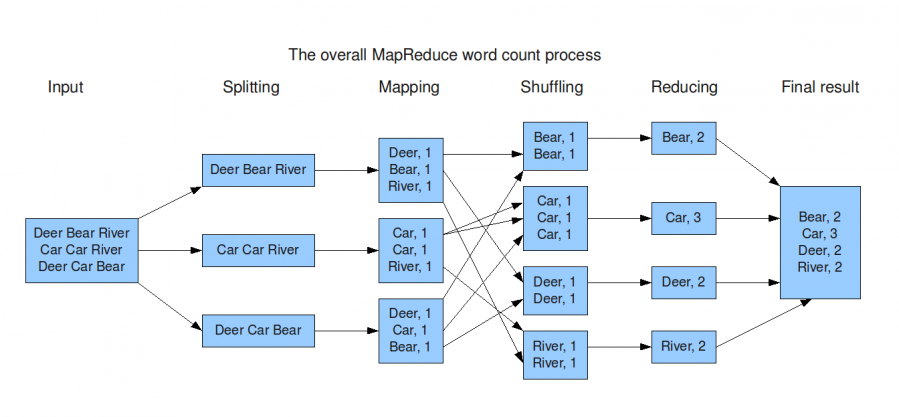
\includegraphics[scale=0.35]{img1}}
		\caption{http://beyondthegeek.com/2016/07/13/mapper-reducer/}
\end{figure}
\end{frame}

\begin{frame}[fragile]
\frametitle{Map Reduce}
\lstset{
	basicstyle=\footnotesize,
	numbers=left,
	numbersep=5pt,
	showtabs=false,
	title=Wortzahl,
	style=customc
}

\begin{lstlisting}
function map(String name, String documentPart):
	for each word w in documentPart:
		emit (w, 1)
 
function reduce(String word, List<Int> partialCounts):
	sum = 0
	for each pc in partialCounts:
		sum += pc
		emit (word, sum)
		
\end{lstlisting}

\end{frame}

\begin{frame}{Hadoop}
\subsection{Hadoop}
\begin{center}
\begin{figure}
		\center{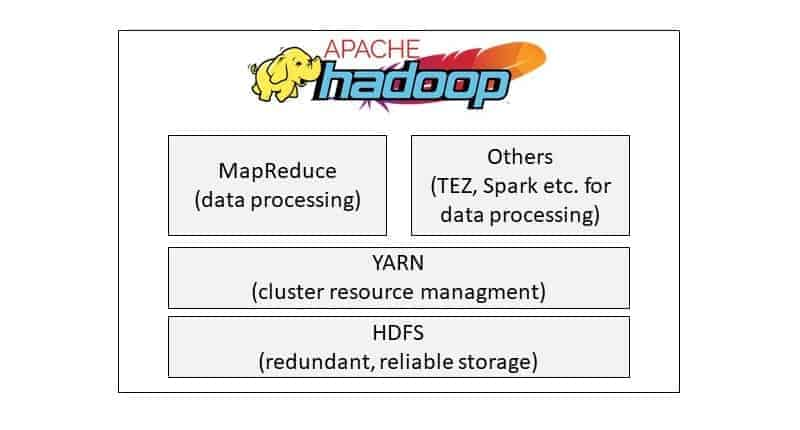
\includegraphics[scale=0.5]{img3}}
\end{figure}
\end{center}
\begin{itemize}
	\item HDFS (Hadoop Distributed File System)
	\item YARN (Yet Another Resource Negotiator)
	\item Map Reduce
\end{itemize}
\end{frame}

\begin{frame}{HDFS}
\begin{figure}
		\center{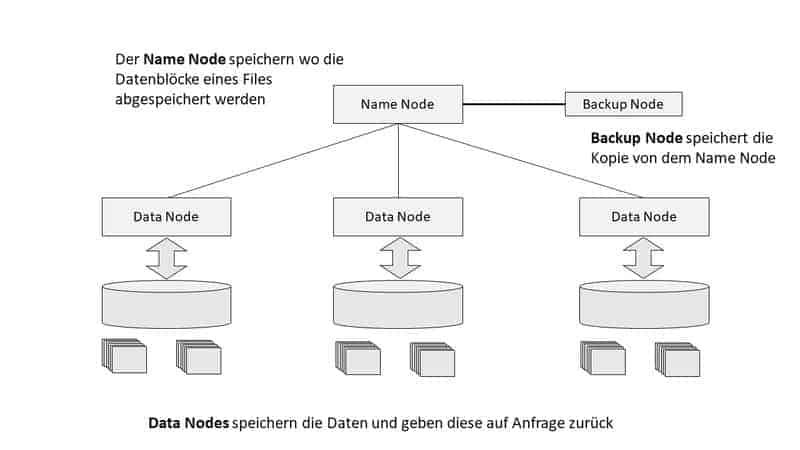
\includegraphics[scale=0.35]{img4}}
		%\caption{https://hadoop.apache.org/hdfs_design.html}
\end{figure}
\end{frame}

%\begin{frame}{Spark}
%\subsection{Spark}
%\end{frame}

\begin{frame}[fragile]
\frametitle{R}
\subsection{R}
Paradigmen:
\begin{itemize}
	\item funktional
	\item dynamisch
	\item objektorientiert
\end{itemize}

%\begin{quotation}
%Everything that exists is an object. Everything that happens is a function call
%\end{quotation}

\lstset{
	language=R,
	basicstyle=\footnotesize,
	numbers=left,
	numbersep=5pt,
	showtabs=false,
	title=R Beispiel Code,
	style=customc
}
\begin{lstlisting}
Gewicht <- c(60, 72, 57, 90, 95, 72)
Groesse <- c(1.75, 1.80, 1.65, 1.90, 1.74, 1.91)
BMI <- Gewicht/ Groesse^2
sum(Gewicht)
length(Gewicht)
sum(Gewicht)/length(Gewicht)
table(Gewicht)
\end{lstlisting}

\end{frame}

\begin{frame}[fragile]
\frametitle{Spark}
\subsection{Spark}
\begin{itemize}
	\item einheitliches In- Memory System 
	\item zur Verarbeitung von enormen Datenmengen geeignet
	\item Framework für Clustercomputing 
	\item Open Source 
	\item Konzept der Resilient Distributed Datasets (RDD)
\end{itemize}
\end{frame}

\begin{frame}
\frametitle{Spark}
\begin{figure}
		\center{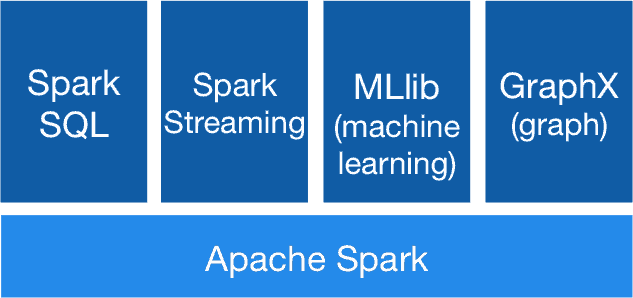
\includegraphics[scale=0.35]{spark}}
		\caption{http://archive.ibmsystemsmag.com/mainframe/business-strategy/bi-and-analytics/dynamic-spark/}
\end{figure}
\end{frame}

\begin{frame}
\frametitle{Zusammenfassung}
\center Schöne neue Welt?
\begin{figure}
		\center{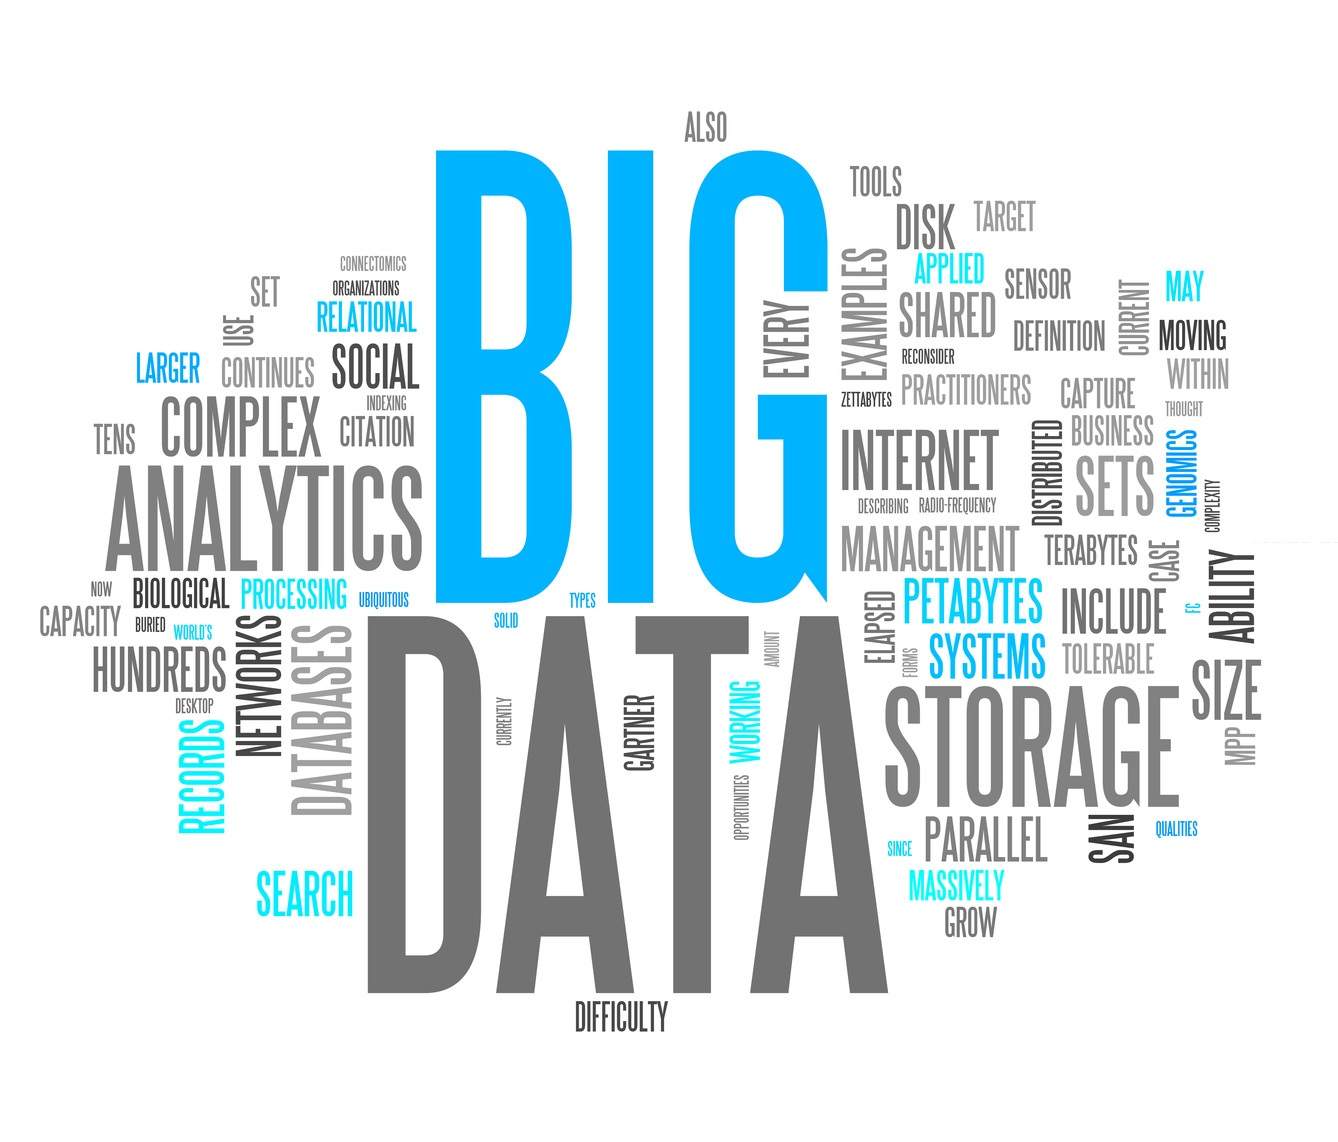
\includegraphics[scale=0.35]{cloud}}
\end{figure}
\end{frame}

\begin{frame}
\frametitle{}
\center Danke für Ihre Aufmerksamkeit!
\end{frame}


\end{document}
